\chapter[2021 August]{August 2021}

\section[2021/08/08]{Sunday, 8 August 2021}

\subsection{STM32F103C8T6}

\subsubsection{Features}

The STM32F103C8T6 microcontroller has the following important features:

\begin{compactitem}
	\item 32-bit ARM Cortex M3 CPU Core with a maximum frequency of 72 MHz and single-cycle multiplication and division.
	\item 64 KB of flash (program) memory organised as 32-bit wide memory cells which may store both program data as well as the program code.
	\item 20KB of SRAM.
	\item 37 GPIOs.
	\item Word size of 32 bits and a half word size of 16 bits
\end{compactitem}

\subsubsection{Startup}

The selection of the system clock occurs when the system starts up. This is the internal 8 MHz oscillator by default. Alternatively, an external oscillator with a frequency in the range 4-16 MHz can be selected on startup. If this external oscillator fails, the RC oscillator will be selected instead by the system. On startup, the system may boot from User Flash, System Memory or the embedded SRAM which is selected using the boot pins. The SysTick timer is a timer that is dedicated for use by the \ac{OS} but may also be used as a downcounter.

\subsubsection{Programming}

The Flash memory embedded in the STM32F103C8T6 can be programmed using either \ac{ICP} or \ac{IAP}. \ac{ICP} involves updating the entirety of Flash memory with the application using the \ac{JTAG} protocol, \ac{SWD} protocol or the boot loader. On the other hand, \ac{IAP} allows the Flash memory to be reprogrammed while the application is running by means of any supported communication interface. The Cortex M3 core integrated two debug ports for both \ac{JTAG} as well as \ac{SWD}.

\pendsign

\section[2021/08/13]{Friday, 13 August 2021}

\subsection{Z-Axis Mount}

It was decided to use aluminium v-slot extrusions as the foundation of the robotic subsystem primarily due to the design flexibility offered this structure. The profile of the extrusion offers considerable stiffness required by the frame structure as well as mounting locations along any position of the structure by means of T-nuts. Furthermore, the v-shape present along the grooves in the extrusion allow the extrusion to be used as a linear guide. The extrusion was not considered as an option for a linear guide in the z-axis assembly due to its comparatively large mass compared to the mass of the z-assembly. However, in comparison to the mass of the x-axis assembly, the mass of the extrusion is much more reasonable and offers greater structural support in comparison to other linear guides such as linear chromed steel rods. The fact that the aluminium v-slot extrusion approach was selected for the rest of the robotic subsystem structure combined with the reasons discussed earlier was considered sufficient to select an aluminium extrusion as the x-axis linear guide. To assist in countering the torque generated about the x-axis by the z-axis assembly, it was decided to use a 2040 aluminium v-slot extrusion as opposed to a 2020 aluminium v-slot extrusion.

Linear motion along the aluminium v-slot extrusion is facilitated by v-slot wheels that run along the v-shaped grooves of the extrusion. Therefore, a need for a component to connect the z-axis assembly to the x-axis aluminium v-slot extrusion arose. The specific requirements of the required component are outlined below:

\begin{compactitem}
	\item The component needs to connect the 4 v-slot wheels positioned to run along the 2040 aluminium v-slot extrusion to the 4 linear bearings through which the linear chromed steel rods of the z-axis assembly run.
	\item The component needs to accommodate the excess movement required by the eccentric nuts used by half of the v-slot wheels.
	\item The component needs to provide mounting points for the timing belt on either side of the component.
	\item The component needs to provide a mounting point for the lead screw nut.
	\item The component needs to accommodate the length of the 8mm diameter to 5mm diameter rigid coupling used to attach the lead screw to the z-axis motor in the z-axis assembly. This accommodation allows the z-axis motor to move lower along the z-axis relative to the fixed linear bearings. This results in a shorter moment arm to the z-axis motor and reduces the torque about the x-axis.
	\item The component needs to be capable of being manufactured using \ac{FDM} 3D printing techniques.
	\item The component needs to support assembly with all of its supporting components.
\end{compactitem}

\begin{figure}[H]
	\centering
	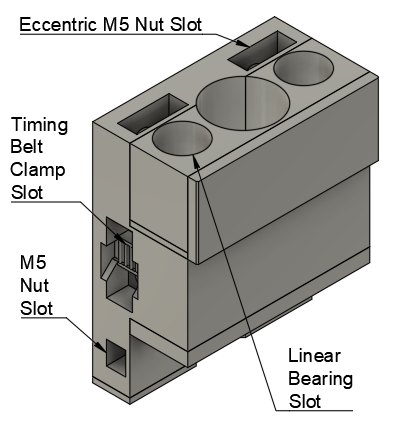
\includegraphics[width=0.35\linewidth]{figures/202108/z-axis-mount.png}
	\caption{Z-axis mount component for the z-axis assembly without supporting components.}
	\label{fig:z-axis-mount}
\end{figure}

\FigRef{fig:z-axis-mount} shows the z-axis mount developed to meet these requirements with various design features relating to these requirements highlighted. The walls of the eccentric spacer measure 1.76 mm and 0.34 mm. That means the bolt may be offset a maximum of 0.71 mm in any direction from the centre of the outer radius of the eccentric spacer which is accommodated in the design by the feature identified as the eccentric M5 nut slot.

The following components are used in conjunction with the z-axis mount:

\begin{compactitem}
	\item 4x delrin solid v-wheels
	\item 4x LM8UU linear bearings
	\item 8mm pitch delrin lead screw nut
	\item 2x eccentric nuts for v-wheels
	\item 4x M5x30 DIN 84 slotted cheese head machine screws
	\item 4x M5 washers
	\item 2x custom designed timing belt clamps
\end{compactitem}

\FigRef{fig:z-axis-mount-assembled} shows the z-axis mount assembled with all the components listed above is shown from an angled perspective from below the component. The 8mm pitch lead screw nut can be seen centred near the bottom of the component. One of the timing belt clamps can be seen placed over the timing belt clamp slot on the side of the z-axis mount.

\begin{figure}[H]
	\centering
	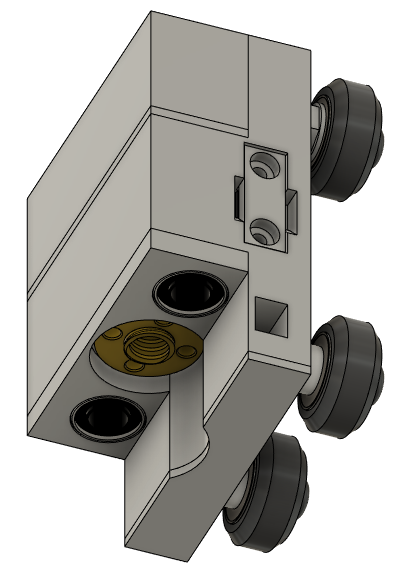
\includegraphics[width=0.3\linewidth]{figures/202108/z-axis-mount-assembled.png}
	\caption{Z-axis mount component for the z-axis assembly with supporting components.}
	\label{fig:z-axis-mount-assembled}
\end{figure}

\subsection{X-Axis Assembly}

For the purposes of this project, the x-axis assembly is defined in a similar manner to the z-axis assembly. Specifically, the x-axis assembly is the collection of components that move linearly along the x-axis when the x-axis drive motor is activated. Similar to the z-axis assembly, a decision needs to be made regarding whether to position the x-axis drive motor as part of the x-axis assembly or not. There is no significant benefit to including the x-axis motor as part of the x-axis assembly either than it potentially reduces the complexity of the x-axis mount which no longer needs to support the motor as well. However, this is offset by the complexity increase in the z-axis mount which would need to include a mounting point for the x-axis motor. Furthermore, mounting the motor in this manner would increase the mass of the x-axis assembly which would require a larger motor with more torque to drive. For these reasons, it was selected to not include the x-axis motor in the x-axis assembly. Note, the x-axis assembly does not include the x-axis linear guide in the form of the 2040 aluminium v-slot extrusion as it does not move when the x-axis drive is activated.

The second design consideration is the selection of the drive mechanism. Again, a lead screw approach was considered against a timing belt based approach. In this situation, the drive mechanism does not need to work directly against gravity as was the case with z-axis assembly. Furthermore, the range of motion of the x-axis assembly is significantly greater than that of the z-axis assembly. Based on these factors, in conjunction with the discussion of the drive mechanisms covered during the z-axis assembly analysis, the timing belt approach was selected. Due to the existence of the v-wheels to connect the z-axis mount to the aluminium extrusion, it was identified as being significantly more complicated to route the timing belt with the flat face parallel to the base plane. However, there were no obvious restrictions in routing the timing belt with the front face parallel to the x-axis aluminium v-slot extrusion. Furthermore, the aluminium v-slot extrusion facilitates the routing of the far side of the belt through the centre of the extrusion. For these reasons, it was decided to route the timing belt in this manner. Therefore, with all of the above considered, the x-axis assembly is defined to only consist of the z-axis mount as well as the z-axis assembly. \FigRef{fig:x-axis-assembly} shows x-axis assembly positioned on the x-axis aluminium v-slot extrusion.

\begin{figure}[H]
	\centering
	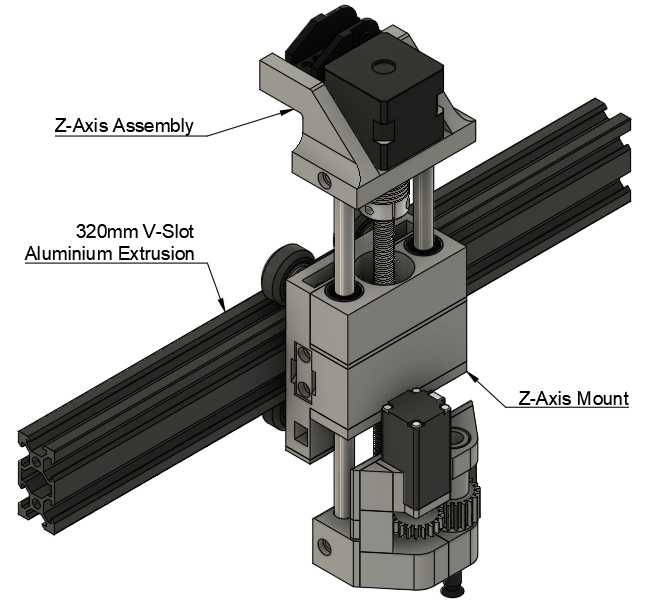
\includegraphics[width=0.8\linewidth]{figures/202108/x-axis-assembly.png}
	\caption{X-axis assembly consisting of the z-axis mount supporting the z-axis assembly.}
	\label{fig:x-axis-assembly}
\end{figure}

\subsection{Y-Axis Assembly}

For the purposes of this project, the y-axis assembly is defined in a similar manner to the z-axis and x-axis assemblies. Specifically, the y-axis assembly is the collection of components that moves linearly along the y-axis when the y-axis drive is activated. At this point in the design, the x-axis assembly is the highest level component of the robotic subsystem. The x-axis assembly runs along the x-axis aluminium v-slot extrusion. In order to introduce linear motion along the y-axis, both of these components need to be translated and therefore will both form part of the y-axis assembly.

In order to facilitate linear motion along the y-axis, linear guides need to be introduced into the design. Again, the most popular two linear guides were considered, namely the linear rail and the linear chromed steel rod. A consideration that applies to the y-axis motion that did not apply to the linear guides used on the other axes is the fact that the y-axis linear guides will always be fixed relative to the robotic structure. Therefore, weight is not a consideration in the selection of the linear guides. Furthermore, it has already been noted that aluminium v-slot extrusions are used to form the frame of the robotic subsystem. These extrusions facilitate simple mounting of linear rails by means of T-nuts. Furthermore, all of the mechanical advantages of the linear rail over the linear chromed steel rod as discussed earlier still apply. Since the y-axis assembly has the greatest mass of any of the moving components, the mechanical advantages offered by the linear rail were considered more relevant here than in earlier parts of the design. V-wheels were also considered as a means of linear motion along the v-slot aluminium extrusion. However, exploration of potential designs using this mechanisms exhibited many issues with routing the timing belt for the x-axis as well as the y-axis. Furthermore, the aluminium spacers would introduce additional length along the x-axis without any increase in the range of motion along the x-axis. 

For these reasons, the linear rail was selected as the linear guide along the y-axis. Furthermore, since both sides of the x-axis aluminium v-slot extrusion need to be supported, it was decided to use two linear rails, one on either side of the x-axis aluminium extrusion. The MGN12H linear bearing acts as the connection between the linear rail and the load item. Therefore, a requirement for two components to connect both ends of the x-axis aluminium extrusion to the MGN12H bearings arose. The requirements of the first component are as follows:

\begin{compactitem}
	\item The component needs to connect the left side of the x-axis 2040 aluminium v-slot extrusion to the left MGN12H linear bearing.
	\item The component needs to provide a mounting point for the 42BYGHW609 stepper motor such that the motor is in a position to drive the x-axis timing belt.
	\item The component needs to provide a timing belt clamping point on both sides of the component for the left y-axis timing belt.
	\item The component needs to facilitate the routing of the x-axis timing belt.
	\item The item needs to provide a mounting point for the end piece of the drag chain to facilitate the routing of wires and tubing originating from the z-axis assembly as well as the 42BYGHW609 stepper motor cables.
	\item The component needs to be capable of being manufactured using \ac{FDM} 3D printing techniques.
\end{compactitem}

\FigRef{fig:x-axis-mount-left} shows the left x-axis mount that was designed to meet these requirements along with indications of the roles of the various parts of the design. Similarly, the requirements of the second component are:

\begin{compactitem}
	\item The component needs to connect the right side of the x-axis 2040 aluminium v-slot extrusion to the right MGN12H linear bearing.
	\item The component needs to provide a mounting point for an idler pulley for a 6mm timing.
	\item The component needs to facilitate the movement of the idler pulley along the x-axis to allow the x-axis timing belt to be adjusted to the correct tension.
	\item The component needs to provide a timing belt clamping point on both sides of the component for the right y-axis timing belt.
	\item The component needs to facilitate the routing of the x-axis timing belt.
	\item The component needs to be capable of being manufactured using \ac{FDM} 3D printing techniques.
\end{compactitem}

\FigRef{fig:x-axis-mount-right} shows the right x-axis mount that was designed to meet these requirements along with indications of the roles of the various parts of the design.

\begin{figure}[H]
	\centering
	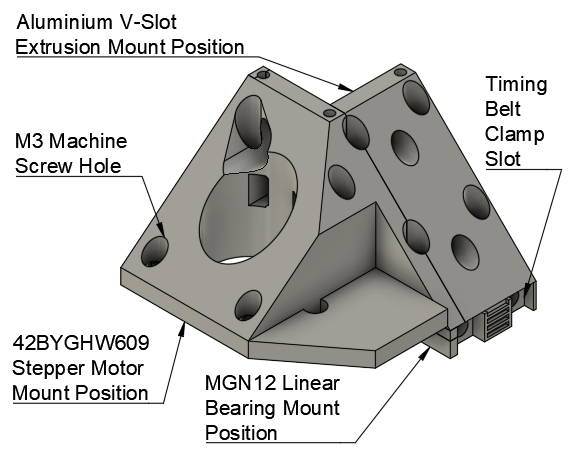
\includegraphics[width=0.45\linewidth]{figures/202108/x-axis-mount-left.png}
	\caption{X-axis assembly left mount.}
	\label{fig:x-axis-mount-left}
\end{figure}

\begin{figure}[H]
	\centering
	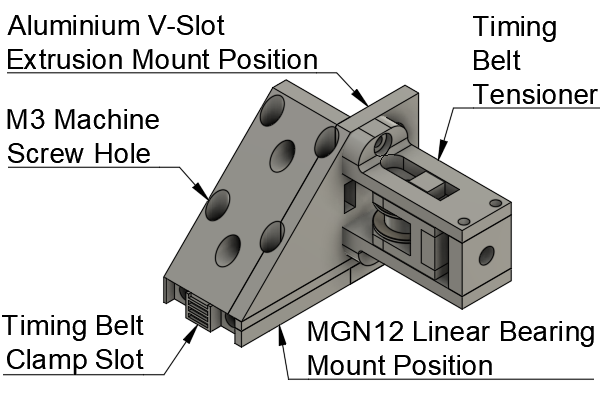
\includegraphics[width=0.4\linewidth]{figures/202108/x-axis-mount-right.png}
	\caption{X-axis assembly right mount.}
	\label{fig:x-axis-mount-right}
\end{figure}

The components that comprise the y-axis assembly are as follows:

\begin{compactitem}
	\item X-axis assembly
	\item X-axis 2040 aluminium v-slot extrusion of length 320mm
	\item Left x-axis mount
	\item Right x-axis mount
	\item 2x MGN12H linear bearings
	\item 42BYGHW609 stepper motor
	\item 4x custom timing belt clamps
	\item 20 tooth GT2 pulley for GT2 timing belt
	\item Idler pulley for 6mm belt
\end{compactitem}

\subsection{Final Assembly}

The highest level component of the robotic subsystem at this point in the design is the y-axis assembly. In order to complete the design, several components still need to be developed, namely the belt tensioners to be used on both the left and right y-axis timing belts as well as the y-axis drive mechanism. The y-axis belt tensioners have identical functions with the only difference being their operation on opposite sides of the robotic subsystem. Therefore, the left and right y-axis timing belt tensioners are mirror images of each other and essentially share the same design. The y-axis belt tensioner component needs to meet the following requirements.

\begin{compactitem}
	\item The component needs to provide a mounting point for the idler pulley for a 6mm timing belt.
	\item The component needs to facilitate mounting of itself to the aluminium v-slot frame of the robotic subsystem.
	\item The component needs to facilitate adjustment of the position of the idler pulley along the y-axis to allow the tension of the y-axis timing belt to be adjusted.
	\item The component needs to be capable of being manufactured using \ac{FDM} 3D printing techniques.
\end{compactitem}

\FigRef{fig:y-axis-belt-tensioner-right} shows the y-axis belt tensioner that was designed to fulfil these requirements on the right side of the robotic subsystem.

\begin{figure}[H]
	\centering
	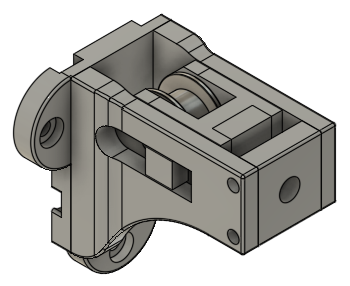
\includegraphics[width=0.4\linewidth]{figures/202108/y-axis-belt-tensioner-right.png}
	\caption{Y-axis belt tensioner for the right drive side.}
	\label{fig:y-axis-belt-tensioner-right}
\end{figure}

The second design that needs to be completed in order to complete the robotic subsystem is the y-axis drive mechanism. The primary requirement of this mechanism is that it needs to be capable of driving the y-axis timing belts on both the left and right side of the robotic subsystem. The obvious basis of this mechanism is to use a dual shaft stepper motor with each shaft used to drive one of the y-axis timing belts. The 42BYGHW920L21B2 stepper motor was selected for this characteristic. Unfortunately, the length of the stepper motor is not sufficient to drive each belt directly off each shaft. Instead it was decided to drive only the left side y-axis timing belt directly off the shaft using a 20 tooth pulley for a 6mm GT2 timing belt with a 5mm bore. In order to drive the right side y-axis timing belt, the torque needs to be transferred from the stepper motor shaft to a pulley connected to the timing belt. It was decided to use an 8mm linear chromed steel rod in order to transfer this torque to a 20 tooth pulley for a 6mm GT2 timing belt with a 8mm bore. An 8mm diameter to 5mm diameter coupling is required to connect the stepper motor shaft to the 8mm linear rod. The rigid coupling is not sufficient to support the linear rod along the drive axis. Therefore, two KP08 8mm pillow block bearings were introduced to support the linear rod. In order to connect the pillow blocks to the aluminium v-slot extrusion frame of the robotic subsystem, two custom connector components needed to be designed. Similarly, a component needed to be designed to connect the 42BYGHW920L21B2 stepper motor to the frame as well. All of the components discussed above form the y-axis drive mechanism which is shown attached to the robotic subsystem in \FigRef{fig:y-axis-drive-assembly}. The final robotic subsystem assembly is shown in \FigRef{fig:final-assembly}.

\begin{figure}[H]
	\centering
	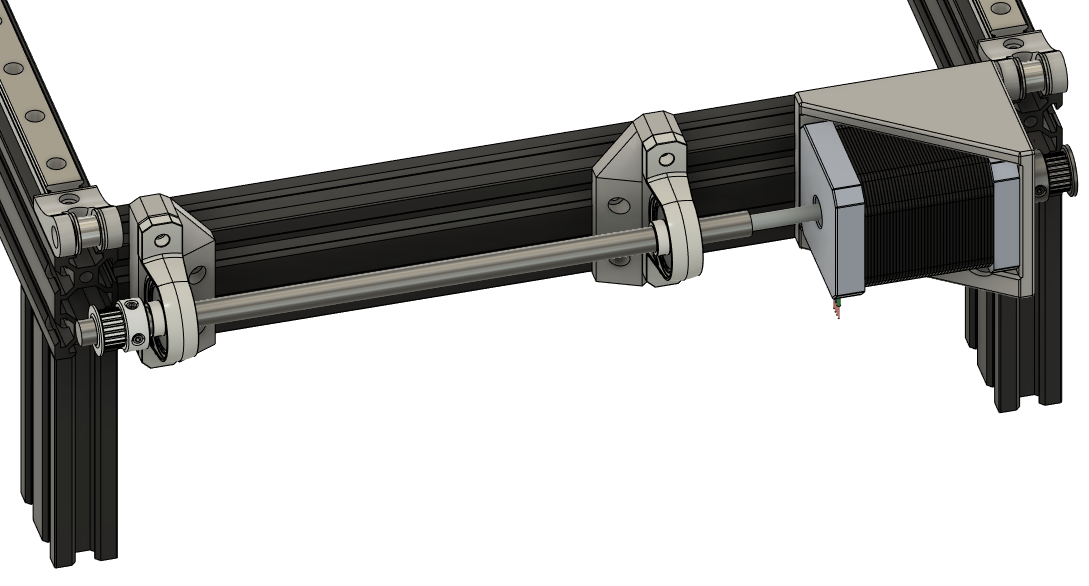
\includegraphics[width=0.7\linewidth]{figures/202108/y-axis-drive-assembly.png}
	\caption{Y-axis drive assembly.}
	\label{fig:y-axis-drive-assembly}
\end{figure}

\begin{figure}[H]
	\centering
	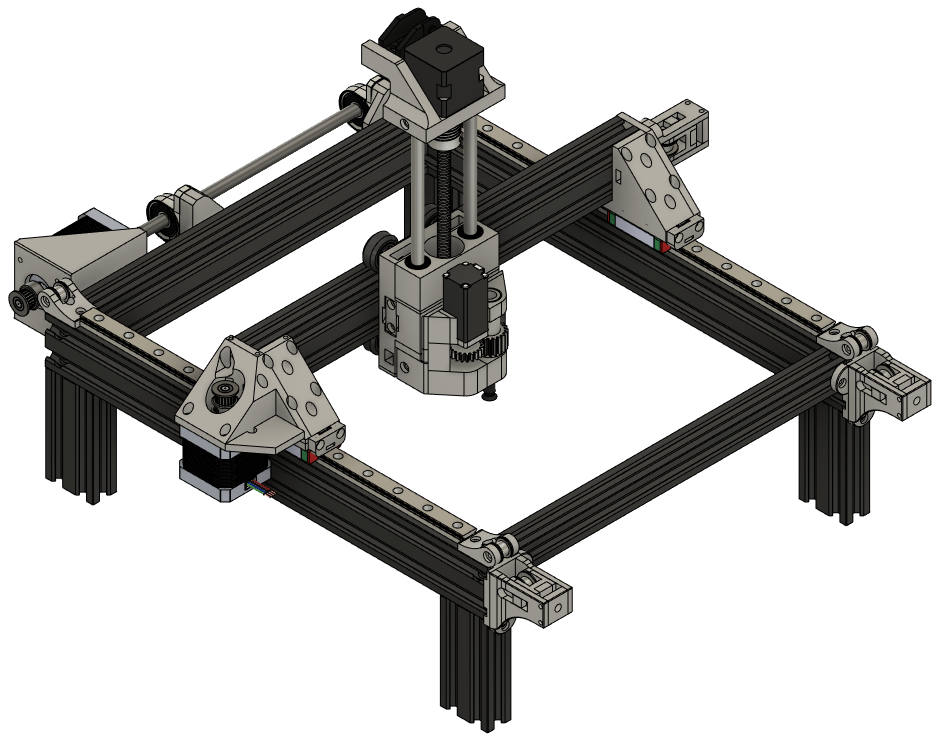
\includegraphics[width=0.9\linewidth]{figures/202108/final-assembly.png}
	\caption{Final robotic subsystem assembly.}
	\label{fig:final-assembly}
\end{figure}

\pendsign